\documentclass[11pt]{article}

\usepackage[margin=1in]{geometry}
\usepackage[T1]{fontenc}
\usepackage{amsmath}
\usepackage{amssymb}
\usepackage{microtype}
\usepackage{xcolor}
\usepackage{listings}
\usepackage{tikz}
\usepackage[
    colorlinks=true,
    linkcolor=blue,
    citecolor=blue,
    urlcolor=blue
]{hyperref}
\usetikzlibrary{arrows.meta,positioning}

\lstset{
    language=Python,
    basicstyle=\ttfamily\small,
    keywordstyle=\color{blue!60!black},
    commentstyle=\color{green!40!black},
    showstringspaces=false,
    breaklines=true,
    frame=single,
    columns=fullflexible
}

\title{Model Parallelism}
\author{}
\date{}

\begin{document}
\maketitle
\tableofcontents
\newpage

\section{What model parallelism divides}

Data parallelism gives different training examples to different ranks. Model
parallelism divides the computation of one model across ranks. For a
transformer, let

\begin{equation}
\begin{split}
X\in\mathbb{R}^{B\times S\times H}
\end{split}
\end{equation}

denote a hidden-state tensor with batch size \(B\), sequence length \(S\), and
hidden size \(H\). Let the model contain \(L\) transformer blocks and, for a
mixture-of-experts model, \(E\) experts. The four forms of model parallelism
divide different axes:

\begin{equation}
\begin{split}
\text{tensor parallelism (TP)}&:\quad \text{features and weight matrices},\\
\text{pipeline parallelism (PP)}&:\quad \text{the }L\text{ transformer blocks},\\
\text{context parallelism (CP)}&:\quad \text{the }S\text{ sequence positions},\\
\text{expert parallelism (EP)}&:\quad \text{the }E\text{ experts}.
\end{split}
\end{equation}

These methods are not four implementations of the same split. Each one cuts a
different part of the computation. OLMo represents their combination with a
named process mesh~\cite{olmo-world-mesh}.

\newpage
\section{The process mesh assigns a job to every rank}

A parallelism degree is the number of ranks used for one kind of split. For a
dense model, a configuration with degrees \(d_{\mathrm{pp}}\),
\(d_{\mathrm{dp}}\), \(d_{\mathrm{cp}}\), and \(d_{\mathrm{tp}}\) requires

\begin{equation}
\begin{split}
W=d_{\mathrm{pp}}d_{\mathrm{dp}}d_{\mathrm{cp}}d_{\mathrm{tp}}
\end{split}
\end{equation}

ranks. \(W\) is the total world size. A missing dimension has degree one.

Consider eight ranks with

\begin{equation}
\begin{split}
d_{\mathrm{pp}}=2,\qquad d_{\mathrm{dp}}=2,\qquad
d_{\mathrm{tp}}=2,\qquad d_{\mathrm{cp}}=1.
\end{split}
\end{equation}

A process mesh is a coordinate system for ranks.  Let \(p\) select a pipeline
stage, \(d\) select a data-parallel batch share, and \(t\) select a
tensor-parallel matrix shard.  Context parallelism has degree one in this
example, so its coordinate is always zero and can be omitted.

OLMo orders these dimensions as pipeline, data, context, and tensor.  With the
degrees above, the rank number is

\begin{equation}
\begin{split}
\operatorname{rank}=4p+2d+t.
\end{split}
\end{equation}

This formula only flattens the three coordinates into one global rank number.
It is a numbering convention, not part of any parallel algorithm.  The formula
gives the complete assignment:

\begin{equation}
\begin{split}
&\begin{array}{c|ccc@{\qquad\qquad}c|ccc}
\text{rank} & p & d & t & \text{rank} & p & d & t\\ \hline
0 & 0 & 0 & 0 & 4 & 1 & 0 & 0\\
1 & 0 & 0 & 1 & 5 & 1 & 0 & 1\\
2 & 0 & 1 & 0 & 6 & 1 & 1 & 0\\
3 & 0 & 1 & 1 & 7 & 1 & 1 & 1
\end{array}
\end{split}
\end{equation}

An extracted submesh specifies which ranks may communicate with one another
for one parallel method.  PyTorch represents those ranks as a \emph{process
group}.  A collective operation such as an all-reduce runs only among the
ranks in the process group.

Holding two coordinates fixed and varying the third produces the following
rank pairs:

\begin{equation}
\begin{split}
&\begin{array}{c|c}
\text{axis varied} & \text{process groups, written as global-rank pairs}\\ \hline
t\ \text{(TP)} & (0,1),\ (2,3),\ (4,5),\ (6,7)\\
d\ \text{(DP)} & (0,2),\ (1,3),\ (4,6),\ (5,7)\\
p\ \text{(PP)} & (0,4),\ (1,5),\ (2,6),\ (3,7)
\end{array}
\end{split}
\end{equation}

Thus there are four separate TP process groups, not one.  On rank 0,
\texttt{get\_tp\_mesh} selects the TP pair \((0,1)\); on rank 2 it selects
\((2,3)\).  Ranks \(i\) and \(i+4\) form a PP pair because changing the
pipeline coordinate \(p\) changes the flattened rank by 4.  Changing the TP
coordinate \(t\) changes it by 1.

The two ranks in a TP pair hold complementary shards of the same layer and
must exchange partial results.  A rank from another DP or PP pair is working
on different data or a different pipeline stage.  Including that rank in the
TP collective would mix unrelated computations.

OLMo constructs the world mesh once and extracts the submesh needed by each
parallel method.  The layer implementations then use the corresponding
process groups for their collective operations:

\begin{lstlisting}[basicstyle=\ttfamily\footnotesize]
world_mesh = build_world_mesh(
    dp=dp_config,
    tp=tp_config,
    cp=cp_config,
    pp=pp_config,
    ep=ep_config,
)

tp_mesh = get_tp_mesh(world_mesh)
cp_mesh = get_cp_mesh(world_mesh)
pp_mesh = get_pp_mesh(world_mesh)
ep_mesh = get_ep_mesh(world_mesh)
\end{lstlisting}

The implementation checks that every enabled degree divides the world size.
It also requires a data-parallel configuration whenever TP, PP, CP, or EP is
enabled~\cite{olmo-world-mesh}.

\section{Tensor parallelism splits matrix multiplication}

For one linear layer,

\begin{equation}
\begin{split}
Y_{if}=\sum_{h=0}^{n_{\mathrm{in}}-1}X_{ih}W_{hf}.
\end{split}
\end{equation}

The index \(i\) identifies an input row.  The input-feature index is
\(h=0,\ldots,n_{\mathrm{in}}-1\), and the output-feature index is
\(f=0,\ldots,n_{\mathrm{out}}-1\).  The multiplication sums over \(h\) and
retains \(f\) in the output.

A \emph{column-wise} split partitions the range of \(f\), assigning one
subrange to each GPU.  Each GPU computes

\begin{equation}
\begin{split}
Y_{if}=\sum_{h=0}^{n_{\mathrm{in}}-1}X_{ih}W_{hf},
\qquad f\text{ in that GPU's assigned range}.
\end{split}
\end{equation}

The sum over \(h\) is complete on each GPU.  Different GPUs produce different
values of \(f\), so their results do not need to be added.

A \emph{row-wise} split partitions the range of \(h\), assigning one subrange
to each GPU.  Each GPU computes a partial value

\begin{equation}
\begin{split}
Z_{\mathrm{local},if}
&=\sum_{h\text{ in that GPU's assigned range}}X_{ih}W_{hf},\\
Y_{if}&=\sum_{\text{GPU in the TP group}}
Z^{(\text{GPU})}_{\mathrm{local},if}.
\end{split}
\end{equation}

Here \(Z_{\mathrm{local}}\) is different on each GPU.  A reduction adds the
corresponding entries of these local tensors.  An \emph{all-reduce with sum}
places the complete sum \(Y\) on every GPU in the TP process group.  A
\emph{reduce-scatter with sum} performs the same addition but gives each GPU
only a different slice of \(Y\).

The equation states the required addition without choosing between these two
collectives.  OLMo's row-wise wrapper makes that choice from its requested
output layout.  A replicated layout uses the complete result, while the
\texttt{Shard(1)} layout used by its transformer blocks keeps the result
sequence-sharded~\cite{olmo-feed-forward,olmo-transformer-block}.

Each GPU produces only part of the same output entry \(Y_{if}\), so a
reduction must add the parts.  This is why the two splits must be
distinguished: column-wise splits the range of \(f\); row-wise splits the
range of \(h\), the index being summed.

\subsection{One transformer MLP}

For a gated feed-forward layer,

\begin{equation}
\begin{split}
Y=\bigl(\phi(XW_1)\odot XW_3\bigr)W_2,
\end{split}
\end{equation}

let \(m_{\mathrm{local}}\) denote the subrange of intermediate-feature indices
assigned to the current GPU.  The first two projections split their output
index:

\begin{equation}
\begin{split}
U[:,m_{\mathrm{local}}]
&=\phi\bigl(XW_1[:,m_{\mathrm{local}}]\bigr)
 \odot XW_3[:,m_{\mathrm{local}}].
\end{split}
\end{equation}

The down projection splits the same index as its summed input index:

\begin{equation}
\begin{split}
Z_{\mathrm{local}}
&=U[:,m_{\mathrm{local}}]W_2[m_{\mathrm{local}},:],\\
Y&=\sum_{\text{GPU in the TP group}}Z_{\mathrm{local}}^{(\text{GPU})}.
\end{split}
\end{equation}

Thus \(W_1\) and \(W_3\) split the intermediate index as an output index,
while \(W_2\) splits it as its summed input index.  The intermediate stays divided
across GPUs; only the down-projection results are added.  The corresponding
OLMo plan is direct~\cite{olmo-feed-forward}:

\begin{lstlisting}[basicstyle=\ttfamily\footnotesize]
parallelize_plan = {
    "w1": colwise_parallel(),
    "w2": rowwise_parallel(output_layouts=output_layout),
    "w3": colwise_parallel(),
}
\end{lstlisting}

After the query, key, and value projections, each tensor can be viewed as
having shape \([B,S,A,D]\), where \(A\) is the number of attention heads and
\(D\) is the number of features in one head.  One head is one fixed value of
the head index: it uses its own length-\(D\) query, key, and value vectors to
compute attention across sequence positions.  The heads are independent until
their outputs are combined by the output projection.

OLMo applies the MLP's TP pattern to these projections.  The query, key, and
value projections are column-wise, so each TP rank computes a subset of the
heads.  The output projection is row-wise and combines the results from those
subsets~\cite{olmo-attention}.

At transformer-block boundaries, OLMo keeps activations sharded along the
sequence axis of the TP group. Layer normalization and dropout then run on the
local sequence slices. OLMo calls this \emph{sequence parallelism}; it is a
companion layout used inside TP and is distinct from the context-parallel mode
described next~\cite{olmo-transformer-block}.

\section{Context parallelism splits a long sequence}

Suppose two CP ranks process one sequence of eight tokens. In the simplest
split, rank 0 holds positions \(0\) through \(3\), and rank 1 holds positions
\(4\) through \(7\). CP divides the sequence activations, not the parameter
tensors; FSDP may separately shard those parameters. The difficulty is
attention: a query in one slice may need keys and values from the other slice.

OLMo supports two ways to exchange the missing attention information.

\subsection{Ring attention}

Each rank keeps its local queries. Key and value blocks circulate around the
CP group. A rank updates its attention result when each key/value block
arrives. After one trip around the ring, every local query has attended to all
allowed positions, but no rank had to store the complete sequence's keys and
values at once.

\subsection{Ulysses attention}

Let the CP group contain \(C\) ranks, and assume that \(A\) is divisible by
\(C\). Initially, each rank holds all \(A\) heads for only its own \(S/C\)
sequence positions:

\begin{equation}
\begin{split}
[B,S/C,A,D],
\end{split}
\end{equation}

This layout cannot run ordinary attention locally: one head needs keys and
values from all \(S\) positions, but each rank has only \(S/C\) positions.
Ulysses exchanges sequence coverage for head coverage. Every rank divides its
\(A\) heads into \(C\) groups and sends one head group to each CP rank. A
receiving rank gets the same head group from all \(C\) sequence slices and
concatenates those slices along the sequence axis. Its new layout is

\begin{equation}
\begin{split}
[B,S,A/C,D],
\end{split}
\end{equation}

The rank now has the complete sequence for \(A/C\) heads, so it computes
ordinary full-sequence attention for those heads. The reverse all-to-all then
does the opposite: each rank divides its \(S\) output positions into \(C\)
chunks and sends one chunk back to each original sequence owner. Each owner
receives all \(A\) head groups for its own \(S/C\) positions, restoring
\([B,S/C,A,D]\). OLMo implements these two layout transformations explicitly
\cite{olmo-context-parallel}.

The model shards input IDs, labels, and positional-encoding buffers with the
same CP assignment before the forward pass. The configuration selects either
the ring method or the Ulysses method~\cite{olmo-transformer-model,olmo-train-config}.

This also explains the connection to the data loader. Ranks in one CP group
receive the same model input. CP divides that input during model computation;
it does not ask the data loader for different examples~\cite{olmo-world-mesh}.

\newpage
\section{Pipeline parallelism splits the block list}

Consider an eight-block transformer and two pipeline stages:

\begin{equation}
\begin{split}
\text{stage 0}:&\quad \text{embedding},\;\text{blocks }0\text{--}3,\\
\text{stage 1}:&\quad \text{blocks }4\text{--}7,\;\text{LM head}.
\end{split}
\label{eq:pipeline-stage-assignment}
\end{equation}

Equation~\eqref{eq:pipeline-stage-assignment} assigns model components to
stages; it is not a computation. OLMo turns each assignment into a smaller
model by copying the transformer and deleting the unassigned components. The
first stage keeps the embedding because it receives token IDs, the last keeps
the language-model head because it produces logits, and each stage keeps only
its assigned block interval.

PyTorch's \texttt{PipelineStage} wraps each smaller model with its stage index,
device, and pipeline process group. The pipeline schedule then sends hidden
states from one stage to the next during forward and sends their gradients in
the reverse direction during backward~\cite{olmo-pipeline-config}.

The batch is divided into microbatches so that different stages can work on
different microbatches at the same time. Each stage stores and updates only
the parameters of its smaller model.

\begin{lstlisting}[basicstyle=\ttfamily\footnotesize]
# Simplified construction of one pipeline stage.
model_part = copy.deepcopy(model)

if not is_first_stage:
    model_part.embeddings = None
if not is_last_stage:
    model_part.lm_head = None

delete_blocks_outside_this_stage(model_part)
stage = PipelineStage(model_part, stage_id, num_stages, device)
\end{lstlisting}

OLMo constructs the configured schedule with the selected number of
microbatches. It does not support tied input and output embeddings across
multiple stages because those weights would be placed in different stage-local
models~\cite{olmo-pipeline-train,olmo-pipeline-config}.

\newpage
\section{Expert parallelism splits the experts}

In a mixture-of-experts layer, a router selects a small number of experts for
each token. Suppose there are four experts and two EP ranks:

\begin{equation}
\begin{split}
\text{rank 0 owns experts }\{0,1\},\qquad
\text{rank 1 owns experts }\{2,3\}.
\end{split}
\end{equation}

A token initially resides on the rank that is processing its input sequence.
Its selected expert may reside on the other rank. The forward pass therefore
has five steps:

\begin{center}
route tokens
\(\longrightarrow\) group by destination rank
\(\longrightarrow\) all-to-all
\(\longrightarrow\) local expert computation
\(\longrightarrow\) reverse all-to-all.
\end{center}

The returned outputs are restored to their original token order and combined
with the router weights. OLMo implements this order as
\texttt{permute\_and\_all\_to\_all}, local expert computation,
\texttt{reverse\_all\_to\_all}, and \texttt{unpermute}
\cite{olmo-parallel-mlp}.

The expert weight tensors are sharded along their expert dimension, so each
rank permanently stores only its local experts~\cite{olmo-expert-mlp}. At the
pinned OLMo revision used here, EP requires HSDP, and TP and EP cannot be
enabled together~\cite{olmo-world-mesh,olmo-parallelize-model}.

\newpage
\section{How OLMo constructs the parallel model}

The process mesh defines rank groups. The model-parallel methods then replace
ordinary local modules with distributed layouts and communication. OLMo
performs these transformations before constructing the optimizer.

\begin{figure}[ht]
\centering
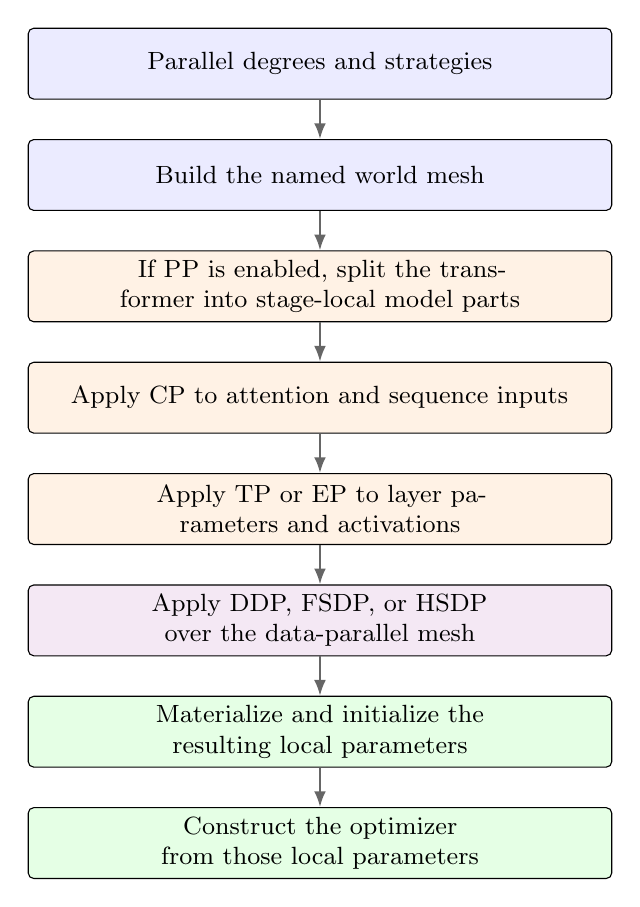
\begin{tikzpicture}[
    node distance=5mm,
    box/.style={draw,rounded corners=2pt,align=center,minimum height=9mm,
        text width=72mm,font=\small,inner sep=3pt},
    arrow/.style={-{Latex[length=2mm]},thick,draw=black!60}
]
\node[box,fill=blue!8] (config) {Parallel degrees and strategies};
\node[box,fill=blue!8,below=of config] (mesh)
    {Build the named world mesh};
\node[box,fill=orange!10,below=of mesh] (pp)
    {If PP is enabled, split the transformer into stage-local model parts};
\node[box,fill=orange!10,below=of pp] (cp)
    {Apply CP to attention and sequence inputs};
\node[box,fill=orange!10,below=of cp] (tp)
    {Apply TP or EP to layer parameters and activations};
\node[box,fill=violet!9,below=of tp] (dp)
    {Apply DDP, FSDP, or HSDP over the data-parallel mesh};
\node[box,fill=green!10,below=of dp] (init)
    {Materialize and initialize the resulting local parameters};
\node[box,fill=green!10,below=of init] (optim)
    {Construct the optimizer from those local parameters};
\draw[arrow] (config) -- (mesh);
\draw[arrow] (mesh) -- (pp);
\draw[arrow] (pp) -- (cp);
\draw[arrow] (cp) -- (tp);
\draw[arrow] (tp) -- (dp);
\draw[arrow] (dp) -- (init);
\draw[arrow] (init) -- (optim);
\end{tikzpicture}
\caption{OLMo transforms the model before training begins. Each optimizer sees
only the parameters represented on its rank after all parallel transformations.}
\label{fig:olmo-parallel-construction}
\end{figure}

The essential control flow is visible in the original implementation
\cite{olmo-parallelize-model,olmo-pipeline-train}:

\begin{lstlisting}[basicstyle=\ttfamily\footnotesize]
world_mesh = build_world_mesh(dp=dp, tp=tp, cp=cp, pp=pp, ep=ep)

# Pipeline training performs this split first.
stages, model_parts = pp.split_model(model, pp_mesh=pp_mesh)

# The shared transformation applies CP, TP or EP, then DP.
model_parts = parallelize_model(
    model_parts,
    world_mesh=world_mesh,
    cp_config=cp,
    tp_config=tp,
    ep_config=ep,
    dp_config=dp,
)

# Each stage builds an optimizer for the parameters it now owns.
optimizers = [optim.build(part) for part in model_parts]
\end{lstlisting}

Without pipeline parallelism, the training loop calls the wrapped model in the
usual way, and its distributed modules perform the required collectives.
With pipeline parallelism, the training loop instead calls the configured
pipeline schedule; that schedule invokes each local stage and performs the
point-to-point transfers between stages.

\begin{thebibliography}{99}

\bibitem{olmo-world-mesh}
Allen Institute for AI.
\newblock OLMo-core process-mesh construction and sub-mesh selection.
\newblock \href{https://github.com/allenai/OLMo-core/blob/92870a33c3fee060d57c3faec52b0b369ece85a6/src/olmo_core/distributed/parallel/__init__.py}{\nolinkurl{src/olmo_core/distributed/parallel/__init__.py}}.

\bibitem{olmo-parallelize-model}
Allen Institute for AI.
\newblock OLMo-core transformer parallelization order.
\newblock \href{https://github.com/allenai/OLMo-core/blob/92870a33c3fee060d57c3faec52b0b369ece85a6/src/olmo_core/train/train_module/transformer/common.py}{\nolinkurl{src/olmo_core/train/train_module/transformer/common.py}}.

\bibitem{olmo-feed-forward}
Allen Institute for AI.
\newblock OLMo-core tensor-parallel feed-forward implementation.
\newblock \href{https://github.com/allenai/OLMo-core/blob/92870a33c3fee060d57c3faec52b0b369ece85a6/src/olmo_core/nn/feed_forward.py}{\nolinkurl{src/olmo_core/nn/feed_forward.py}}.

\bibitem{olmo-attention}
Allen Institute for AI.
\newblock OLMo-core tensor- and context-parallel attention implementation.
\newblock \href{https://github.com/allenai/OLMo-core/blob/92870a33c3fee060d57c3faec52b0b369ece85a6/src/olmo_core/nn/attention/__init__.py}{\nolinkurl{src/olmo_core/nn/attention/__init__.py}}.

\bibitem{olmo-transformer-block}
Allen Institute for AI.
\newblock OLMo-core transformer-block parallelization.
\newblock \href{https://github.com/allenai/OLMo-core/blob/92870a33c3fee060d57c3faec52b0b369ece85a6/src/olmo_core/nn/transformer/block.py}{\nolinkurl{src/olmo_core/nn/transformer/block.py}}.

\bibitem{olmo-context-parallel}
Allen Institute for AI.
\newblock OLMo-core context-parallel layout transformations.
\newblock \href{https://github.com/allenai/OLMo-core/blob/92870a33c3fee060d57c3faec52b0b369ece85a6/src/olmo_core/distributed/parallel/context_parallel.py}{\nolinkurl{src/olmo_core/distributed/parallel/context_parallel.py}}.

\bibitem{olmo-transformer-model}
Allen Institute for AI.
\newblock OLMo-core transformer model input and parallelization logic.
\newblock \href{https://github.com/allenai/OLMo-core/blob/92870a33c3fee060d57c3faec52b0b369ece85a6/src/olmo_core/nn/transformer/model.py}{\nolinkurl{src/olmo_core/nn/transformer/model.py}}.

\bibitem{olmo-train-config}
Allen Institute for AI.
\newblock OLMo-core transformer training configuration.
\newblock \href{https://github.com/allenai/OLMo-core/blob/92870a33c3fee060d57c3faec52b0b369ece85a6/src/olmo_core/train/train_module/transformer/config.py}{\nolinkurl{src/olmo_core/train/train_module/transformer/config.py}}.

\bibitem{olmo-pipeline-config}
Allen Institute for AI.
\newblock OLMo-core transformer pipeline splitting.
\newblock \href{https://github.com/allenai/OLMo-core/blob/92870a33c3fee060d57c3faec52b0b369ece85a6/src/olmo_core/train/train_module/transformer/config.py}{\nolinkurl{src/olmo_core/train/train_module/transformer/config.py}}.

\bibitem{olmo-pipeline-train}
Allen Institute for AI.
\newblock OLMo-core pipeline training module.
\newblock \href{https://github.com/allenai/OLMo-core/blob/92870a33c3fee060d57c3faec52b0b369ece85a6/src/olmo_core/train/train_module/transformer/pipeline_train_module.py}{\nolinkurl{src/olmo_core/train/train_module/transformer/pipeline_train_module.py}}.

\bibitem{olmo-expert-mlp}
Allen Institute for AI.
\newblock OLMo-core expert-weight sharding.
\newblock \href{https://github.com/allenai/OLMo-core/blob/92870a33c3fee060d57c3faec52b0b369ece85a6/src/olmo_core/nn/moe/mlp.py}{\nolinkurl{src/olmo_core/nn/moe/mlp.py}}.

\bibitem{olmo-parallel-mlp}
Allen Institute for AI.
\newblock OLMo-core expert token routing and all-to-all communication.
\newblock \href{https://github.com/allenai/OLMo-core/blob/92870a33c3fee060d57c3faec52b0b369ece85a6/src/olmo_core/nn/moe/parallel_mlp.py}{\nolinkurl{src/olmo_core/nn/moe/parallel_mlp.py}}.

\end{thebibliography}

\end{document}
